%% March 2018
%%%%%%%%%%%%%%%%%%%%%%%%%%%%%%%%%%%%%%%%%%%%%%%%%%%%%%%%%%%%%%%%%%%%%%%%%%%%
% AGUJournalTemplate.tex: this template file is for articles formatted with LaTeX
%
% This file includes commands and instructions
% given in the order necessary to produce a final output that will
% satisfy AGU requirements, including customized APA reference formatting.
%
% You may copy this file and give it your
% article name, and enter your text.
%
%
% Step 1: Set the \documentclass
%
% There are two options for article format:
%
% PLEASE USE THE DRAFT OPTION TO SUBMIT YOUR PAPERS.
% The draft option produces double spaced output.
%

%% To submit your paper:
\documentclass[draft]{agujournal2018}
\usepackage{apacite}
\usepackage{url} %this package should fix any errors with URLs in refs.
%%%%%%%
% As of 2018 we recommend use of the TrackChanges package to mark revisions.
% The trackchanges package adds five new LaTeX commands:
%
%  \note[editor]{The note}
%  \annote[editor]{Text to annotate}{The note}
%  \add[editor]{Text to add}
%  \remove[editor]{Text to remove}
%  \change[editor]{Text to remove}{Text to add}
%
% complete documentation is here: http://trackchanges.sourceforge.net/
%%%%%%%


%% Enter journal name below.
%% Choose from this list of Journals:
%
% JGR: Atmospheres
% JGR: Biogeosciences
% JGR: Earth Surface
% JGR: Oceans
% JGR: Planets
% JGR: Solid Earth
% JGR: Space Physics
% Global Biogeochemical Cycles
% Geophysical Research Letters
% Paleoceanography and Paleoclimatology
% Radio Science
% Reviews of Geophysics
% Tectonics
% Space Weather
% Water Resources Research
% Geochemistry, Geophysics, Geosystems
% Journal of Advances in Modeling Earth Systems (JAMES)
% Earth's Future
% Earth and Space Science
% Geohealth
%
% ie, \journalname{Water Resources Research}

\journalname{Departamento de Estatística}


% tightlist command for lists without linebreak
\providecommand{\tightlist}{%
  \setlength{\itemsep}{0pt}\setlength{\parskip}{0pt}}



\usepackage{soulutf8}
\usepackage{hyperref}
\usepackage{caption, graphicx, subfig, epstopdf, enumitem}

\begin{document}


%% ------------------------------------------------------------------------ %%
%  Title
%
% (A title should be specific, informative, and brief. Use
% abbreviations only if they are defined in the abstract. Titles that
% start with general keywords then specific terms are optimized in
% searches)
%
%% ------------------------------------------------------------------------ %%

% Example: \title{This is a test title}

\title{Vendas de jogos de videogames}

%% ------------------------------------------------------------------------ %%
%
%  AUTHORS AND AFFILIATIONS
%
%% ------------------------------------------------------------------------ %%

% Authors are individuals who have significantly contributed to the
% research and preparation of the article. Group authors are allowed, if
% each author in the group is separately identified in an appendix.)

% List authors by first name or initial followed by last name and
% separated by commas. Use \affil{} to number affiliations, and
% \thanks{} for author notes.
% Additional author notes should be indicated with \thanks{} (for
% example, for current addresses).

% Example: \authors{A. B. Author\affil{1}\thanks{Current address, Antartica}, B. C. Author\affil{2,3}, and D. E.
% Author\affil{3,4}\thanks{Also funded by Monsanto.}}

\authors{
Guilherme da Rocha Cunha
\affil{1}
\thanks{Matrícula: 221030007}
Gabriel Maurício Chagas Silva
\affil{1}
\thanks{Matrícula: 221017097}
Gustavo Almeida Valentim
\affil{1}
\thanks{Matrícula: 202014468}
}


% \affiliation{1}{First Affiliation}
% \affiliation{2}{Second Affiliation}
% \affiliation{3}{Third Affiliation}
% \affiliation{4}{Fourth Affiliation}

\affiliation{1}{Universidade de Brasília, CIC - Depto de Ciências da
Computação}
%(repeat as many times as is necessary)

%% Corresponding Author:
% Corresponding author mailing address and e-mail address:

% (include name and email addresses of the corresponding author.  More
% than one corresponding author is allowed in this LaTeX file and for
% publication; but only one corresponding author is allowed in our
% editorial system.)

% Example: \correspondingauthor{First and Last Name}{email@address.edu}

%% Keypoints, final entry on title page.

%  List up to three key points (at least one is required)
%  Key Points summarize the main points and conclusions of the article
%  Each must be 100 characters or less with no special characters or punctuation

% Example:
% \begin{keypoints}
% \item	List up to three key points (at least one is required)
% \item	Key Points summarize the main points and conclusions of the article
% \item	Each must be 100 characters or less with no special characters or punctuation
% \end{keypoints}

\begin{keypoints}
\item Exercitar os conhecimentos adquiridos ao longo do curso ``EST0001
- COMPUTAÇÃO EM ESTATÍSTICA 1''.
\end{keypoints}

%% ------------------------------------------------------------------------ %%
%
%  ABSTRACT
%
% A good abstract will begin with a short description of the problem
% being addressed, briefly describe the new data or analyses, then
% briefly states the main conclusion(s) and how they are supported and
% uncertainties.
%% ------------------------------------------------------------------------ %%

%% \begin{abstract} starts the second page

\begin{abstract}
Este documento consiste no relatório do trabalho final da disciplina
``EST0001 - COMPUTAÇÃO EM ESTATÍSTICA 1''. Nele se encontra o
desenvolvimento da análise do conjunto de dados escolhido pelo grupo
utilizando as ferramentas provenientes do R Markdown e das bibliotecas
ggplot, tidyverse e dentre outras.
\end{abstract}
\section{Introdução e Objetivos}

A indústria de jogos de videogames emergiu como uma força poderosa e
inovadora no cenário do entretenimento global, experimentando um
crescimento exponencial ao longo das últimas décadas. Este projeto final
da disciplina ``EST0001 - COMPUTAÇÃO EM ESTATÍSTICA 1'' propõe uma
análise estatística aprofundada das vendas de jogos de videogames,
visando aplicar os conhecimentos adquiridos durante o curso para
explorar padrões, tendências e insights relevantes presentes em um
conjunto de dados específico.

\subsection{Contextualização}

A escolha de investigar o mercado de videogames como tema central desta
análise é respaldada pela sua importância econômica e cultural. No
contexto da constante evolução tecnológica e do crescente interesse pela
mídia digital, compreender as dinâmicas das vendas de jogos torna-se não
apenas uma necessidade para os desenvolvedores e distribuidores, mas
também um elemento crucial para os investidores que buscam entender e
explorar oportunidades neste setor em expansão.

A indústria de jogos não é apenas um mercado; é um ecossistema dinâmico
que reflete as preferências e comportamentos em constante mutação dos
consumidores. A análise estatística desse cenário não apenas ilumina as
tendências emergentes, mas também oferece uma visão valiosa sobre a
interseção entre arte, tecnologia e negócios.

\subsection{Objetivos}

O cerne deste projeto é a aplicação prática dos conhecimentos adquiridos
ao longo do curso ``EST0001 - COMPUTAÇÃO EM ESTATÍSTICA 1''. Os
objetivos específicos delineados para esta análise são os seguintes:

\begin{itemize}
  \item \textbf{Análise Exploratória dos Dados: } Realizar uma investigação profunda do conjunto de dados escolhido, buscando identificar padrões, tendências e características distintivas no mercado de jogos de videogame. Isso inclui uma compreensão abrangente das variáveis envolvidas, tais como plataformas, gêneros, regiões e períodos temporais.  
  
  \item \textbf{Utilização de Ferramenta R: } Aplicar habilidades de programação em R, explorando as funcionalidades das bibliotecas ggplot e tidyverse para criar visualizações impactantes. O uso dessas ferramentas não apenas facilita a interpretação dos dados, mas também permite uma comunicação eficaz das descobertas, tornando a análise acessível e informativa.  
  
  \item \textbf{Extração de Insights Estratégicos: } Além de descrever o panorama atual do mercado, o projeto visa extrair insights estatísticos que possam orientar decisões estratégicas na indústria de videogames. Isso pode incluir recomendações sobre lançamentos de jogos, segmentação de público-alvo ou até mesmo projeções de vendas com base em padrões históricos identificados.

\end{itemize}

Em síntese, este projeto propõe-se a ser mais do que uma simples análise
estatística; é uma exploração profunda e multidimensional do universo
das vendas de jogos de videogames, destacando a interseção entre ciência
de dados e uma das formas mais dinâmicas de expressão artística e
cultural da atualidade.

\section{Metodologia}

O banco de dados escolhido para análise foi o ``Venda de Jogos de
Videogames''
(\url{https://www.kaggle.com/code/rafa84miranda/vendas-de-jogos-de-videogames}).
Ao ler e carregar o banco de dados \texttt{vgsales.csv}, a tabela
retornada contém variáveis que não são relevantes para este projeto que
visa o impacto da indústria dos videogames no cenário global, tais como
\texttt{NA\_Sales}, \texttt{EU\_Sales}, \texttt{JP\_Sales} e
\texttt{Other\_Sales} que focam em regiões específicas do globo,
diferente da variável \texttt{Global\_Sales} que condiz melhor com o
intuito do projeto. Para isso, a utilização da biblioteca tidy e dplyr,
ambas do pacote tidyverse, foram essencias para o desenvolvimento da
análise.

Transformando o banco de dados em um dado do tipo tibble e usando as
opções de modalagem providas pelo dplyr, foi possível o descarte dos
dados não significantes e a simplificação da tabela para melhor
aproveitamento.

Com o conjunto de dados alinhado com os objetivos do trabalho, sua
análise parte do uso da biblioteca ggplot que, por sua vez, permite
melhor visualização e compreensão das relações existentes entre
variáveis via gráficos de diferentes tipos.

\section{Análise de Dados}

Desde 1950, cientistas da computação construíam sistemas de jogos
simples para principalmente demonstrarem o poder dos computadores da
época. Com o passar dos anos, o poder computacional veio crescendo
proporcionalmente, resultando na criação do primeiro jogo de arcade e do
primeiro console de videogame doméstico no início da década de 1970 nos
Estados Unidos, onde marca o nascimento da indústria moderna dos jogos.
Com a ``democratização'' dos jogos de videogame, em 1972, o jogo Pong da
Atari se torna o primeiro jogo de arcade bem sucedido, iniciando assim a
era da crescente popularização de videogames.

\begin{figure}[h]
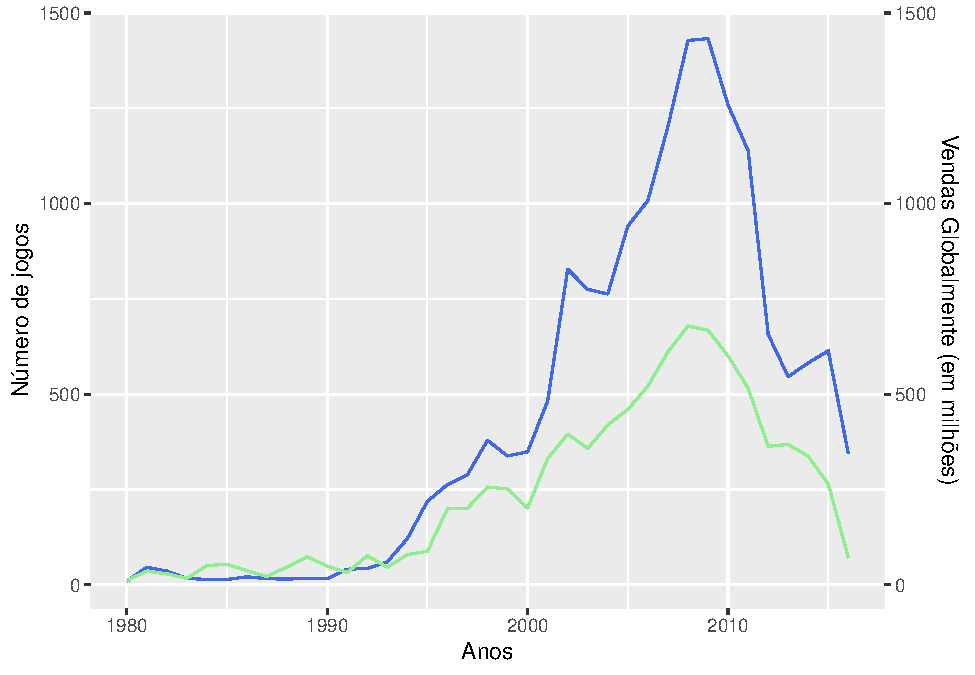
\includegraphics{vendas_de_jogos_de_videogames_files/figure-latex/unnamed-chunk-4-1} \caption{Popularidade dos jogos no decorrer dos anos}\label{fig:unnamed-chunk-4}
\end{figure}

O gráfico acima demonstra a relação proporcionalmente direta entre o
número de jogos desenvolvidos/produzidos no ano, representado pela linha
azul, e a popularidade (medida pela vendas globais), por sua vez
representada pela linha verde.

Graças aos contínuos avanços tecnológicos, novas plataformas, capazes de
executarem videogames cada vez mais complexos computacionalmente, foram
criadas.

\begin{figure}[h]
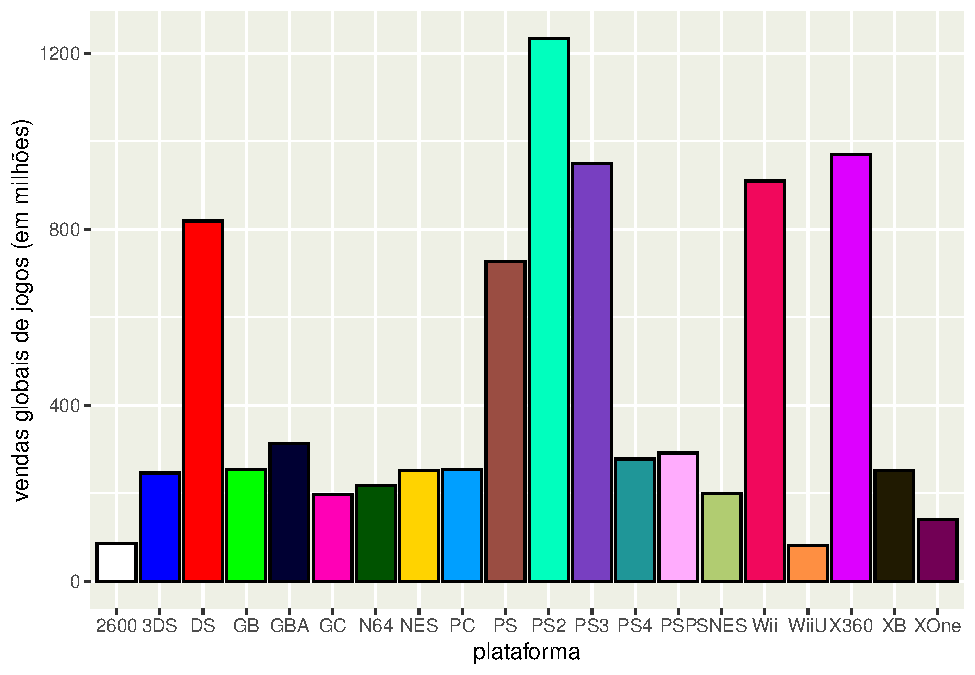
\includegraphics{vendas_de_jogos_de_videogames_files/figure-latex/unnamed-chunk-5-1} \caption{Plataformas mais populares}\label{fig:unnamed-chunk-5}
\end{figure}

No gráfico acima, onde estão as 20 plataformas de jogos mais populeres
historicamente, observa-se que quem lidera é o PlayStation2, levando em
consideração a quantidade de jogos vendidos globalmente.

Como é de se esperar, videogames acabam abordando diferentes temas,
formas de jogabilidades e dentre outras mecânicas. Com isso, os gêneros
dos jogos acabam também influenciando as tendências do mercado, assim
como as plataformas nas quais esses gêneros podem ser explorados ao
máximo.

\begin{figure}[h]
\subfloat[Popularidade dos gêneros no decorrer dos anos\label{fig:unnamed-chunk-6-1}]{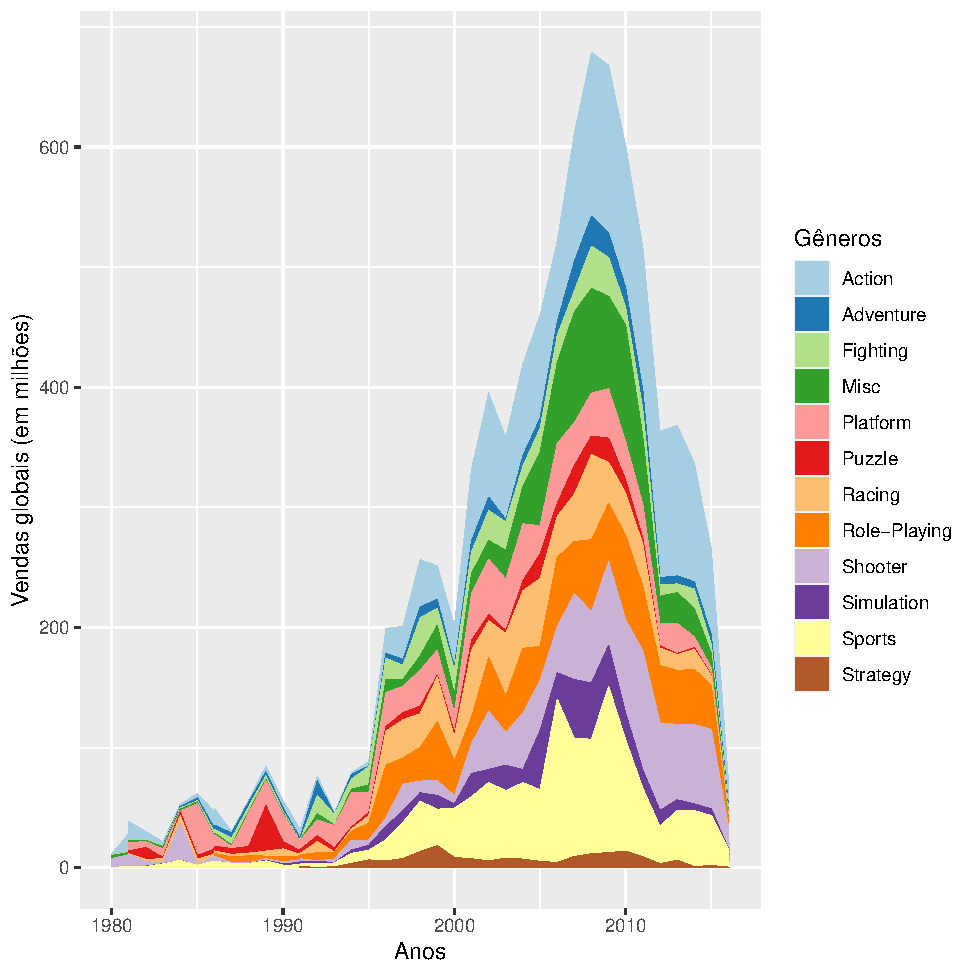
\includegraphics[width=.55\linewidth,]{vendas_de_jogos_de_videogames_files/figure-latex/unnamed-chunk-6-1} }\subfloat[Popularidade dos gêneros nas plataformas mais populares\label{fig:unnamed-chunk-6-2}]{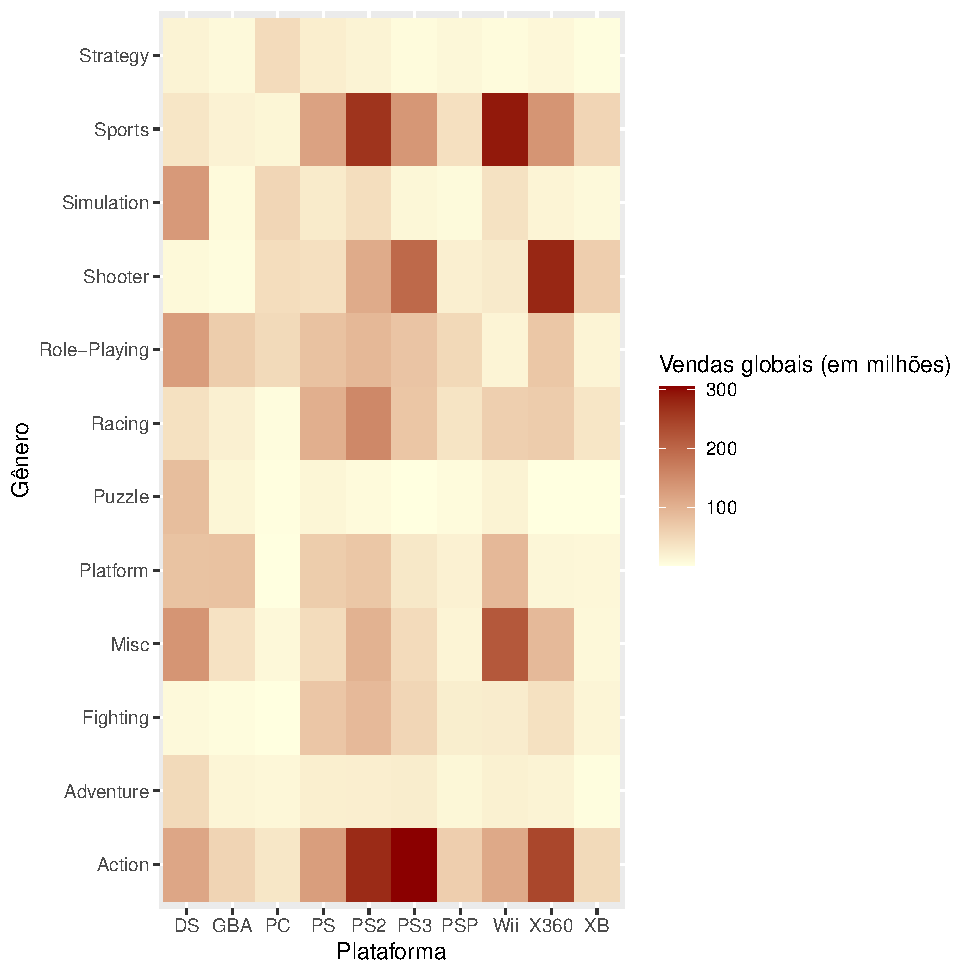
\includegraphics[width=.55\linewidth,]{vendas_de_jogos_de_videogames_files/figure-latex/unnamed-chunk-6-2} }\caption{Influência dos gêneros de jogos}\label{fig:unnamed-chunk-6}
\end{figure}

No gráfico (b), vemos a evolução das vendas de jogos divididas pelo
gênero. Naturalmente, todos os gêneros tiveram um aumento de vendas por
volta do anos 1990, pois é nessa época que os videogames começaram a se
difundir mais e se consolidaram na indústria global de entreternimento.
É nessa época que consoles clássicos como o SNES e o PlayStation1 são
lançados. É interessante notar como desde os anos 1980 até os anos 2010
o genêro de Ação sempre foi o mais popular entre os jogos, e conforme o
tempo passa essa distância só aumentou. O gráfico de ``mapa de calor''
(a) mostra os gêneros de jogsos mais populares para as 10 plataformas
mais populares. É interessanre notar como a genêro de Ação costuma ser o
mais popular entre todas as plataformas, com exceção do Nintendo Wii,
onde o genêro de Esportes é visivelmente o mais popular. Tal fato se
deve a própria natureza do console Wii, que necessita de mais movimento
geral do corpo para os jogos, algo intensamente explorado pela própria
da Nintendo, principalmente no marketing, que juntamente com outras
empresas, desenvolveram diversos jogos de esportes se aproveitando da
movimentação dos jogadores. Outro ponto interessante e o grande número
de jogos de Tiro vendidos para o Xbox360, algo que acreditamos que se
deve a franquia de jogos Halo, uma série de jogos de tiro em primeira
pessoa bastante popular, produzida exclusivamente para os consoles da
Microsoft. Além disso, observa-se ainda que muitos jogos de Esportes
também foram vendidos para o PlayStation2, o que crêemos se explicar
pela popularização das franquias de jogos de futebol FIFA e PES a partir
dos anos 2000.

Assim como a Atari, novas empresas surgiram e obtiveram grande sucesso
com suas inovações e produtos, se destacando no mercado.

\begin{figure}[h]
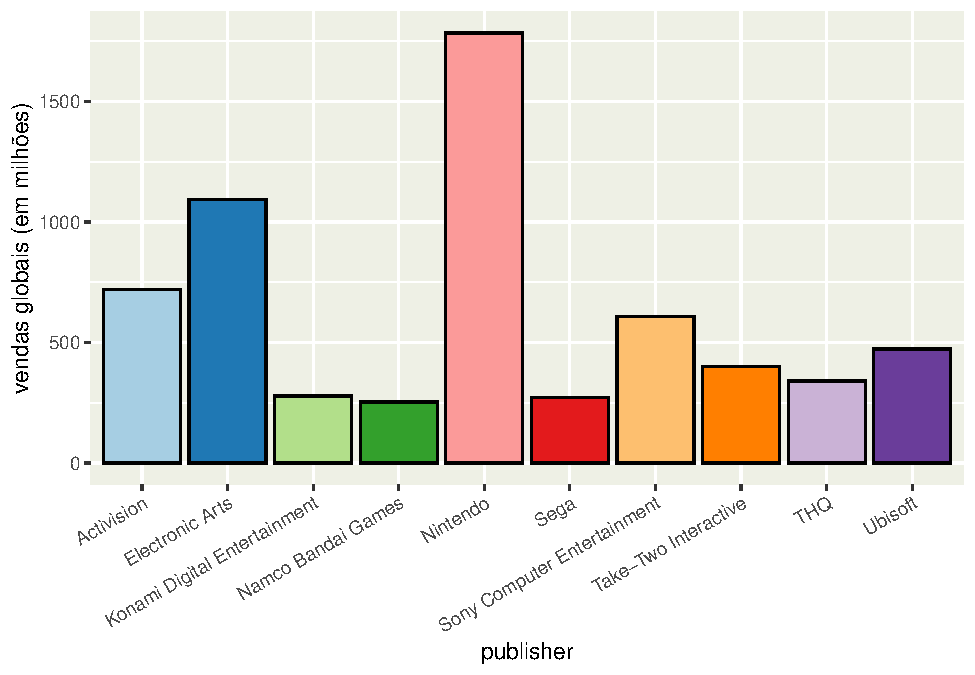
\includegraphics{vendas_de_jogos_de_videogames_files/figure-latex/unnamed-chunk-7-1} \caption{Popularidade das empresas}\label{fig:unnamed-chunk-7}
\end{figure}

\newpage

\begin{figure}[h]
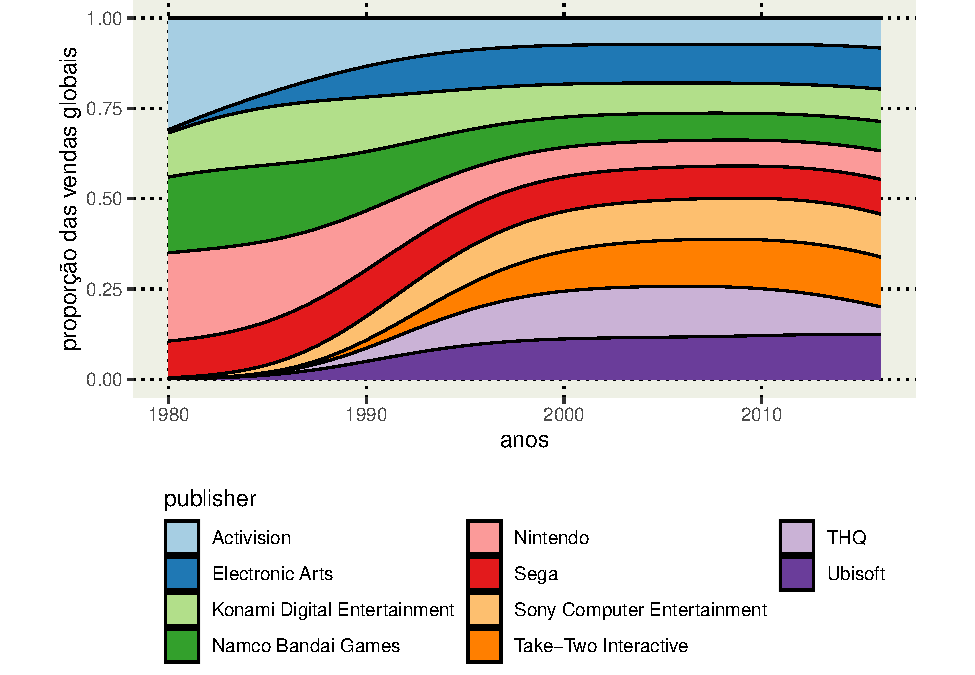
\includegraphics{vendas_de_jogos_de_videogames_files/figure-latex/unnamed-chunk-8-1} \caption{Popularidade das empresas ao longo dos anos}\label{fig:unnamed-chunk-8}
\end{figure}

Nos gráficos acima, onde estão as 10 empresas de jogos mais populares
historicamente, é possível observar a Nintendo no topo, levando em
consideração a quantidade de jogos vendidos globalmente. Além disso,
podemos observar a evolução da presença dessas companhias no mercado,
onde vemos que empresas como Actvision, Namco e Nintendo dominavam nos
anos 1980, mas passaram a dividir espaço com empresas mais novas que
ganharam mais destaque a partir dos anos 1990 e 2000, como a Ubisoft,THQ
e Take-Two Interactive.

\newpage

O conjunto de dados escolhido ranqueia os jogos mais vendidos de 1980
até 2016. Quando reunimos o top 100 jogos mais vendidos, conseguimos
observar algumas relações.

\begin{figure}[h]
\subfloat[Principais empresas do Top 100 jogos\label{fig:unnamed-chunk-9-1}]{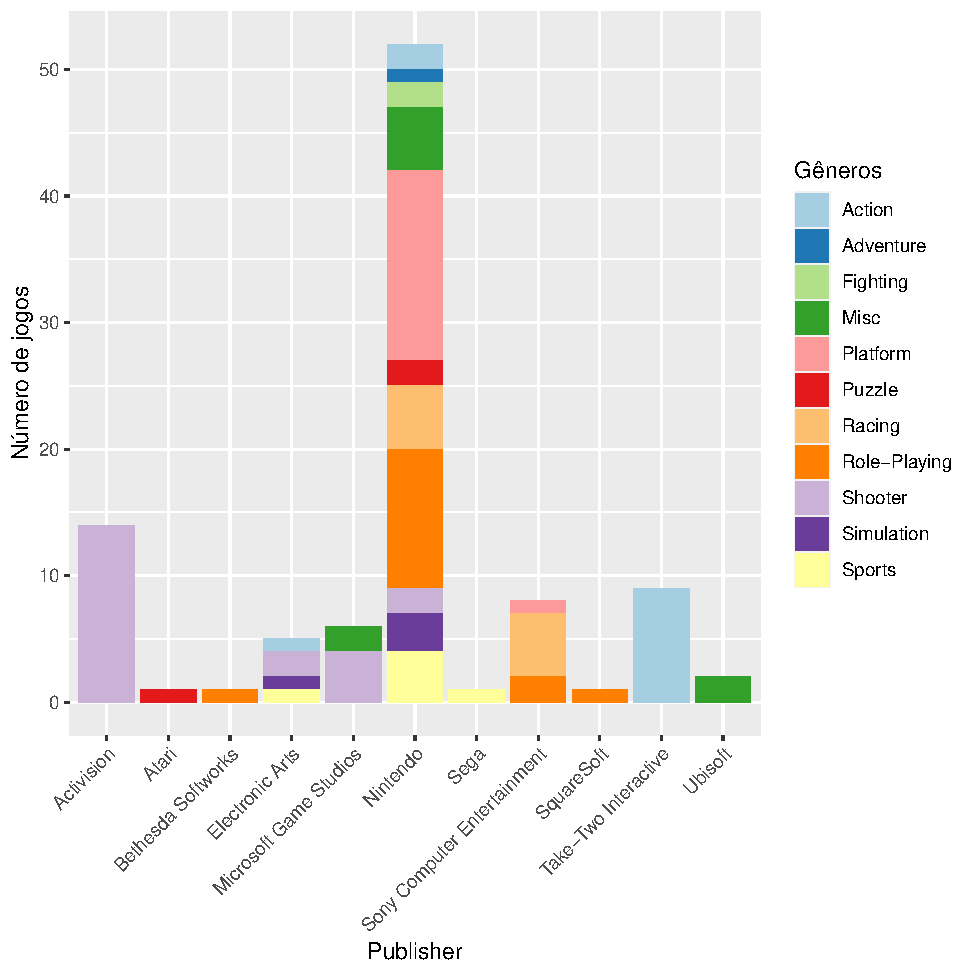
\includegraphics[width=.55\linewidth,]{vendas_de_jogos_de_videogames_files/figure-latex/unnamed-chunk-9-1} }\subfloat[Proporção de gêneros no Top 100 jogos\label{fig:unnamed-chunk-9-2}]{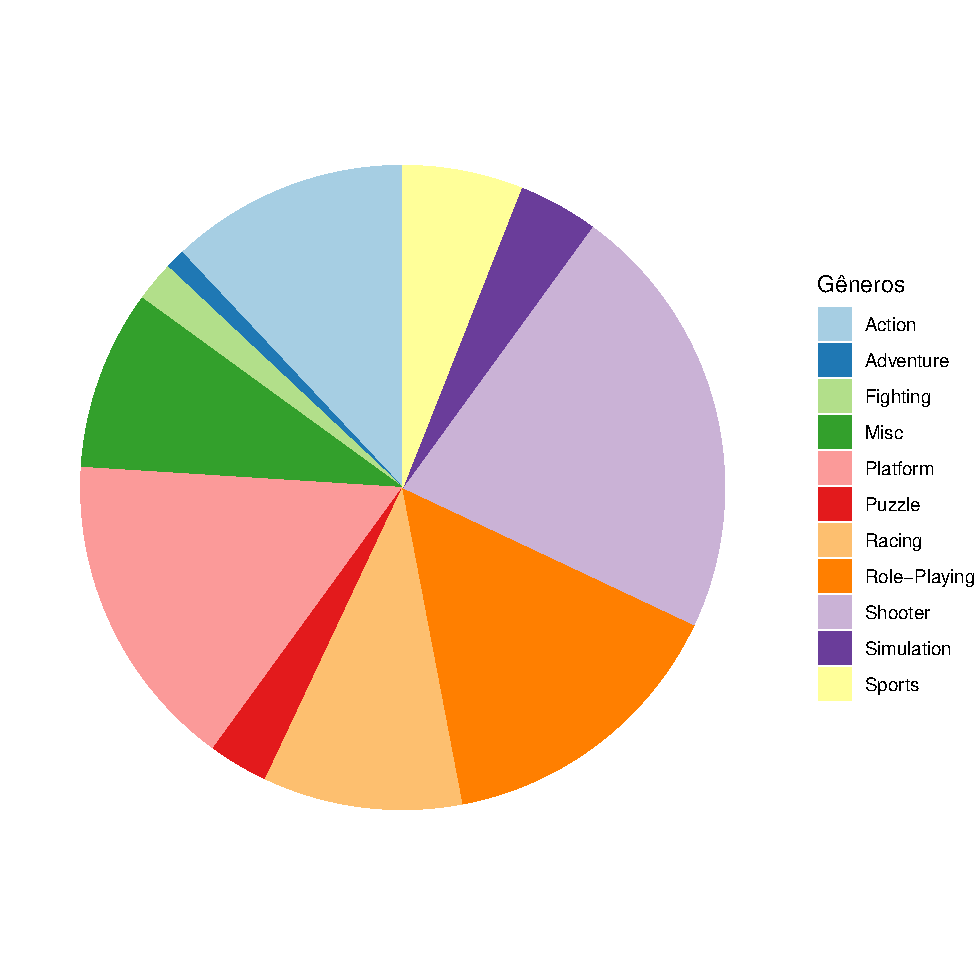
\includegraphics[width=.55\linewidth,]{vendas_de_jogos_de_videogames_files/figure-latex/unnamed-chunk-9-2} }\caption{Relação dos top 100 jogos}\label{fig:unnamed-chunk-9}
\end{figure}

No gráfico (a), nota-se o tamanho sucesso da Nintendo no mercado dos
videogames. Vários de seus produtos estão contidos no top 100, além de
ser uma empresa que aborda vários gêneros diferentes em suas obras, ao
contrário de outras empresas que se ``especializam'' em certos gêneros,
como a Activision e Take-Two Interactive. No gráfico (b), podemos
observar as tendências dos jogos mais bem sucedidos serem dos gêneros de
``Shooter'', ``Platform'', ``Action'' ou ``Role-playing''. É fácil
perceber esta tendência ao analisarmos grandes clássicos do mundo dos
jogos, como a franquia Pokémon (Role-playing), Super Mário (Platform),
Grand Theft Auto (Action) e Call of Duty (Shooter).

\section{Conclusão}

Este projeto, dedicado à análise estatística das vendas de jogos de
videogames no âmbito da disciplina ``EST0001 - COMPUTAÇÃO EM ESTATÍSTICA
1'', culmina em uma compilação meticulosa e profunda das descobertas,
destacando insights relevantes que transcendem simples números. Ao
imergir nas complexidades do mercado de videogames, abordando suas
particularidades e nuances, esta investigação visa contribuir
substancialmente para uma compreensão mais abrangente das dinâmicas
desse setor multifacetado.

Ao longo desta jornada analítica, procuramos não apenas quantificar
vendas, identificar padrões ou traçar correlações, mas, de maneira mais
significativa, compreender o tecido intrincado que compõe a indústria de
jogos eletrônicos. A constatação de que por trás de cada ponto de dado
há uma narrativa sobre preferências culturais, avanços tecnológicos e
estratégias de mercado adiciona uma camada de profundidade à nossa
análise.

As ferramentas estatísticas e de programação em R foram mais do que
meros instrumentos; tornaram-se aliadas na exploração deste universo
digital. Ao integrar a riqueza de técnicas estatísticas com a
flexibilidade do R, alcançamos não apenas uma abordagem abrangente, mas
uma imersão nas sutilezas que compõem o mercado de jogos.

Este projeto não é uma mera formalidade acadêmica; é uma contribuição
tangível para o entendimento prático e pragmático do mercado de
videogames. À medida que apresentamos nossos achados, reconhecemos que
esses insights não são apenas informações, mas bússolas valiosas para
tomadas de decisão informadas.

Em síntese, a jornada por meio das vendas de jogos de videogames,
respaldada por métodos estatísticos, transcendeu expectativas. Os
resultados não são apenas uma resposta aos desafios propostos pela
disciplina, mas uma incursão profunda em um domínio vibrante, onde a
arte, a tecnologia e a estatística convergem. Que este trabalho não
apenas preencha uma lacuna no conhecimento, mas também inspire futuras
explorações e reflexões sobre a dinâmica inebriante da indústria de
videogames.

\bibliography{agutest.bib}


\end{document}
